\chapter{Challenges} \label{apdx:evaluation}

\begin{minted}{javascript} 
[

  {
    id: "connect", 
    title: "Getting started",
    description: "Get connected to the browser you've set up.",
    instruction: "Connect to a browser."
  },

  {
    id: "playlibrary",
    title: "Play your collection.",
    description: "Now we're connected, it would be nice to get some music
        playing. Try playing all the songs in your collection."
  },
  
  {
    id: "skipsong",
    title: "Skip to the next song.",
    description:"Let's pretend you're bored of this one. Skip to the next
        song."
  },
  
  {
    id: "startshuffle",
    title: "Turn on shuffle.",
    description:"How about mixing things up a bit? Try turning on shuffle."
  },
  
  {
    id: "search",
    title: "Searching for music.",
    description: "Search for and play the song \"Shuffle\" by Bombay Bicycle
        Club",
    instruction: "Play \"Shuffle\" by Bombay Bicycle Club"
  },
  
  {
    id: "viewalbum",
    title: "Viewing an album",
    description: "There's a song called \"Eyesdown\" by Bonobo in your
        favourites, and you want to check out the rest of the album.",
    instruction: "Open the album for Eyesdown."
  },
  
  {
    id: "addalbumtoplaylist",
    title: "Add something to a playlist",
    description: "You decide that you like the whole album, and want to
        save it in a playlist.",
    instruction: "Add all of \"Black Sands\" to a playlist."
  }

]
\end{minted}

\chapter{Navigation Graphs}

\begin{figure*}
\centering
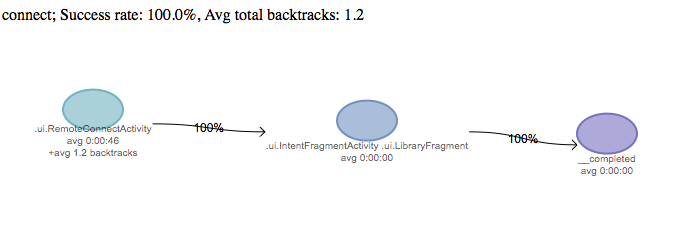
\includegraphics[angle=90,height=\textheight]{images/results/connect}
\end{figure*}

\begin{figure*}
\centering
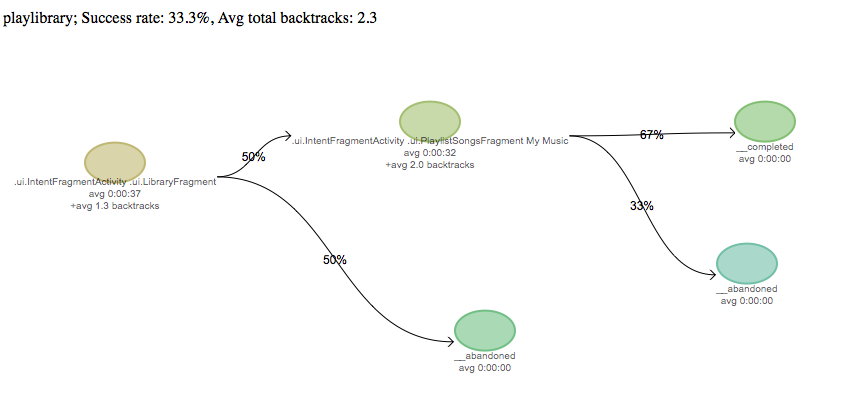
\includegraphics[angle=90,height=\textheight]{images/results/playlibrary}
\end{figure*}

\begin{figure*}
\centering
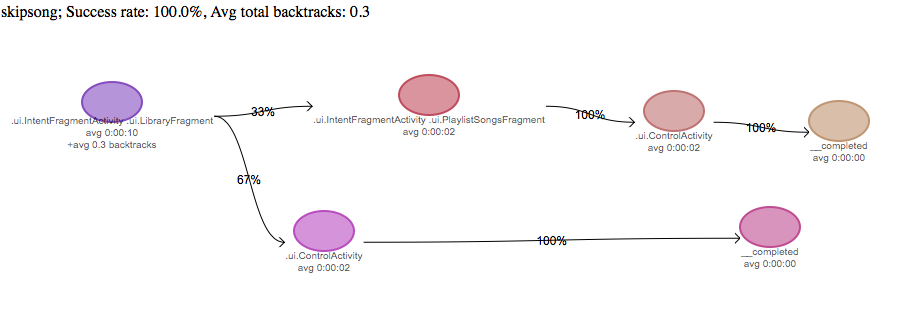
\includegraphics[angle=90,height=\textheight]{images/results/skipsong}
\end{figure*}

\begin{figure*}
\centering
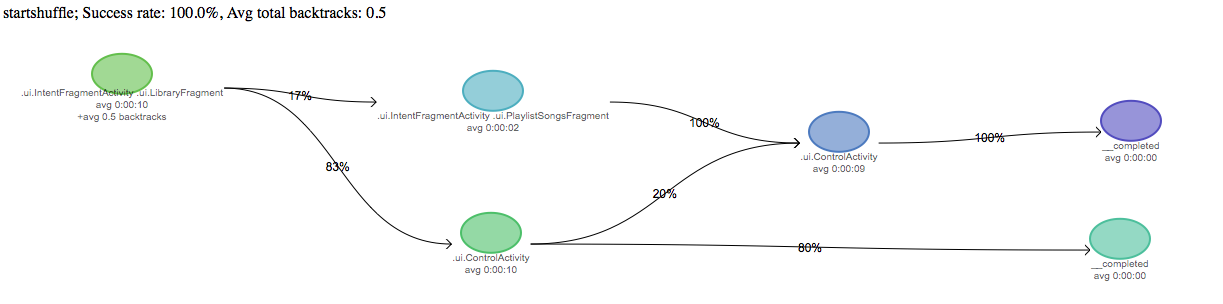
\includegraphics[angle=90,height=\textheight]{images/results/startshuffle}
\end{figure*}

\begin{figure*}
\centering
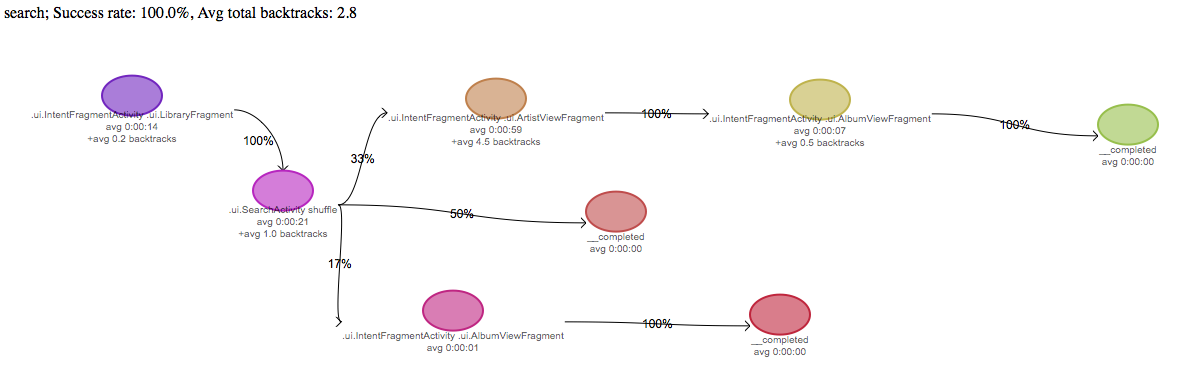
\includegraphics[angle=90,height=\textheight]{images/results/search}
\end{figure*}

\begin{figure*}
\centering
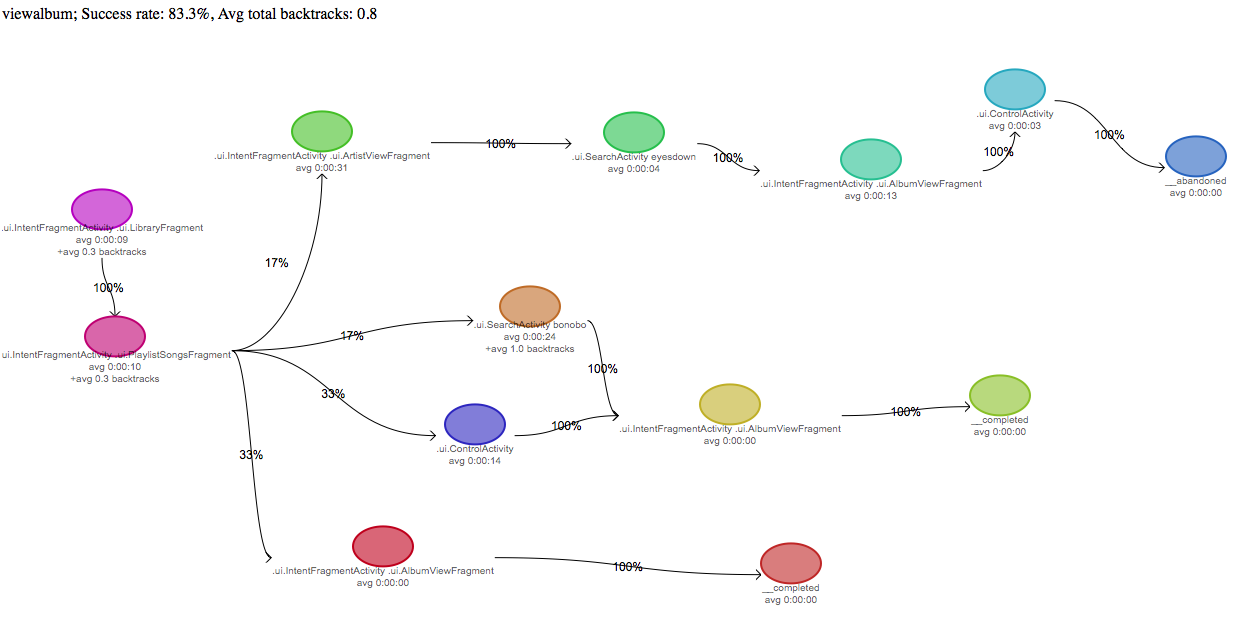
\includegraphics[angle=90,height=\textheight]{images/results/viewalbum}
\end{figure*}

\begin{figure*}
\centering
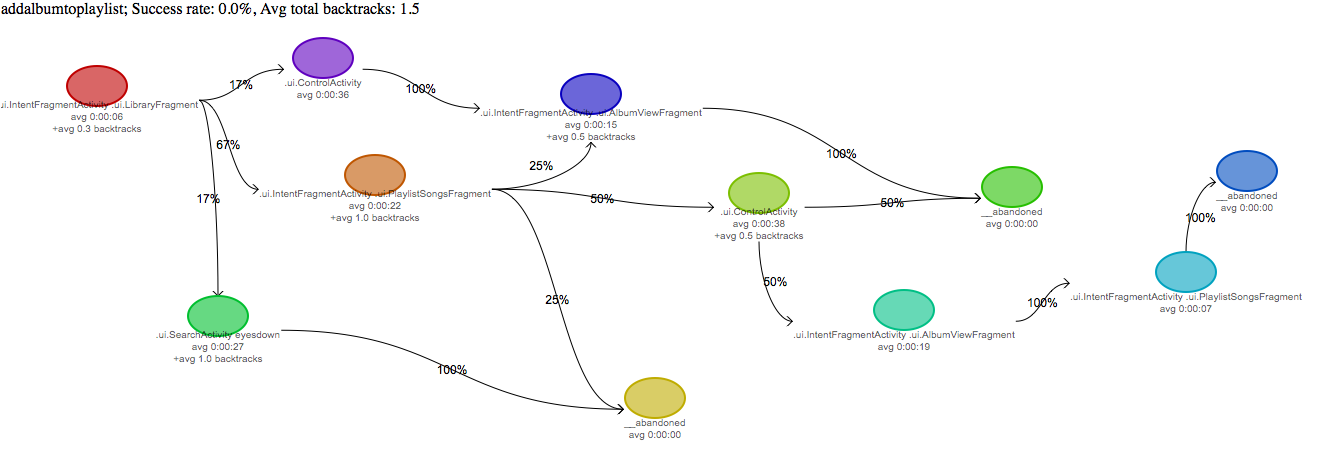
\includegraphics[angle=90,height=\textheight]{images/results/addalbumtoplaylist}
\end{figure*}

